\documentclass{ximera}
\title{Equipotentiaaloppervlakken}
\author{Daan Lipkens}

\begin{document}
\begin{abstract}
    Vlakken van gelijke potentiaal in een elektrisch veld, en hun verband met de veldlijnen.
\end{abstract}
\maketitle

\section{Definitie}
In een homogeen veld geldt $V = E \cdot d$: alle punten die zich op dezelfde afstand $d$ van de negatieve plaat bevinden, hebben dus \textbf{dezelfde potentiaal}.

\begin{definition}[title={Equipotentiaaloppervlak}]\nl
Een \textbf{equipotentiaaloppervlak} is een oppervlak gevormd door alle punten met dezelfde potentiaal.
\end{definition}

In een homogeen veld zijn de equipotentiaaloppervlakken vlakken die evenwijdig lopen met de platen.

\begin{center}
    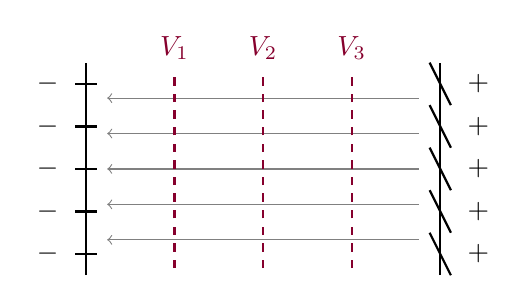
\begin{tikzpicture}[scale=0.9]
        \draw[thick] (0,-1.5) -- (0,1.5);
        \draw[thick] (5,-1.5) -- (5,1.5);
        \foreach \y in {-1.2,-0.6,0,0.6,1.2} {
            \draw[thick] (-0.15,\y) -- (0.15,\y);
            \node[left] at (-0.25,\y) {$-$};
            \draw[thick] (4.85,\y+0.3) -- (5.15,\y-0.3);
            \node[right] at (5.25,\y) {$+$};
        }
        \foreach \y in {-1,-0.5,0,0.5,1} {
            \draw[->, gray] (4.7,\y) -- (0.3,\y);
        }
        \foreach \x in {1.25,2.5,3.75} {
            \draw[dashed, purple!70!black, thick] (\x,-1.4) -- (\x,1.4);
        }
        \node[purple!70!black, above] at (1.25,1.4) {$V_1$};
        \node[purple!70!black, above] at (2.5,1.4) {$V_2$};
        \node[purple!70!black, above] at (3.75,1.4) {$V_3$};
    \end{tikzpicture}
\end{center}

\begin{remark}[title={Belangrijke eigenschap}]\nl
De veldlijnen staan steeds \textbf{loodrecht} op de equipotentiaaloppervlakken. Dit geldt niet enkel voor een homogeen veld, maar voor \emph{elk} elektrisch veld.
\end{remark}

\begin{hint}
    Je kan equipotentiaallijnen vergelijken met hoogtelijnen op een stafkaart: elke lijn verbindt punten op dezelfde hoogte, en het pad van sterkste stijging (de helling) staat er steeds loodrecht op — net zoals veldlijnen loodrecht staan op de equipotentiaaloppervlakken.
\end{hint}

\section{Potentiaal bepalen in een punt}
Om de potentiaal in een willekeurig punt van een veld te bepalen, plaats je een (proef)lading $Q$ in dat punt en bereken je de verhouding $E_{\text{pot}}/Q$. Zoals eerder vermeld hangt deze verhouding niet af van de gekozen testlading $Q$ zelf, maar enkel van het veld en de plaats van het punt in dat veld.

\begin{question}
    Twee punten $A$ en $B$ bevinden zich op eenzelfde equipotentiaaloppervlak van een elektrisch veld. Een lading wordt van $A$ naar $B$ verplaatst. Wat gebeurt er met haar potentiële energie tijdens deze verplaatsing?

    \begin{multipleChoice}
        \choice{Ze wordt groter.}
        \choice{Ze wordt kleiner.}
        \choice[correct]{Ze blijft gelijk.}
        \choice{Er zijn te weinig gegevens om dit te bepalen.}
    \end{multipleChoice}

    \begin{hint}
        Wat is het verband tussen de potentiaal $V$ in een punt en de potentiële energie van een lading $Q$ in dat punt? Verandert dit verband als $A$ en $B$ dezelfde potentiaal hebben?
    \end{hint}

    \begin{solution}\nl
        Omdat $A$ en $B$ op hetzelfde equipotentiaaloppervlak liggen, geldt $V_A = V_B$. Aangezien $E_{\text{pot}} = Q \cdot V$ en de lading $Q$ niet verandert tijdens de verplaatsing, blijft ook de potentiële energie gelijk.
    \end{solution}
\end{question}

\end{document}